\section{Soluci\'on Propuesta}

\begin{frame}{Soluci\'on Propuesta}
Para el desarrollo de la interfaz que permita reconocer comandos de voz, se opt\'o por una metodolog\'ia
de trabajo de c\'odigo abierto, lo cual incluye las tecnolog{\'\i}as y el proceso de desarrollo 
utilizados.

La metodolog\'ia adoptada permiti\'o utilizar un proyecto
existente como punto de partida, al cual se a\~nadi\'o soporte para comandos de voz. 
\end{frame}

\begin{frame}{Soluci\'on Propuesta (2)}
\framesubtitle{Tecnolog\'ia a utilizar}

\textbf{TamTam Edit}
es una aplicaci\'on, parte del compendio de 
actividades\footnote{Una Actividad, es una aplicaci\'on en el entorno 
de escritorio \emph{Sugar}} conocido como \emph{TamTam} desarrollado para la computadora 
XO\footnote{La XO, es una computadora port\'atil de bajo costo y consumo desarrollada por el proyecto
\emph{One Laptop Per Child}}, que proporciona una interfaz intuitiva para crear, modificar y organizar 
notas ubicadas en pistas virtuales utilizando el ratón y el teclado.

\begin{figure}[H]
\centering
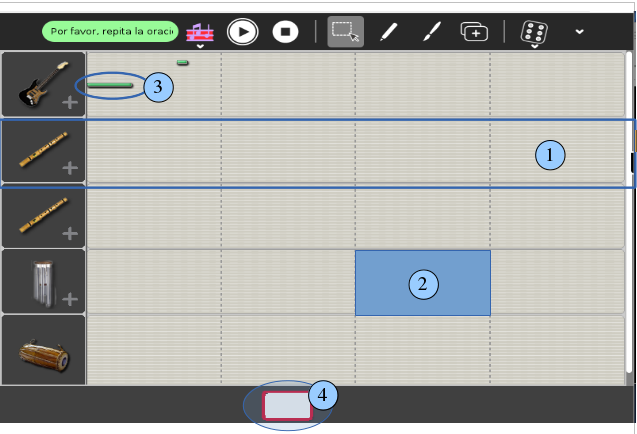
\includegraphics[width=0.7\textwidth]{./graphics/ui-tamtam-edit.png}
\caption{Interfaz de \emph{Tamtam Edit} y sus elementos principales.}
\label{figure:ui-tamtam}
\end{figure}
\end{frame}

\begin{frame}{Soluci\'on Propuesta (3)}
\framesubtitle{Tecnolog\'ia a utilizar}
\textbf{PocketSphinx}
es un motor de reconocimiento del habla de c\'odigo abierto orientado a la optimizaci\'on del rendimiento
y la portabilidad. 
Considerando la naturaleza de este trabajo, adem\'as de las caracter{\'\i}sticas del \foreign{hardware} y el 
\foreign{software} de la \foreign{XO}, se ha elegido esta librer\'ia para implementar la 
interfaz alternativa a la ofrecida por \emph{TamTam Edit}.

\foreign{PocketSphinx} ofrece una implementaci\'on del proceso presentado anteriormente. La implementaci\'on utilizada
como parte de este trabajo se presenta en la siguiente figura.

\begin{figure}[H] 
\centering
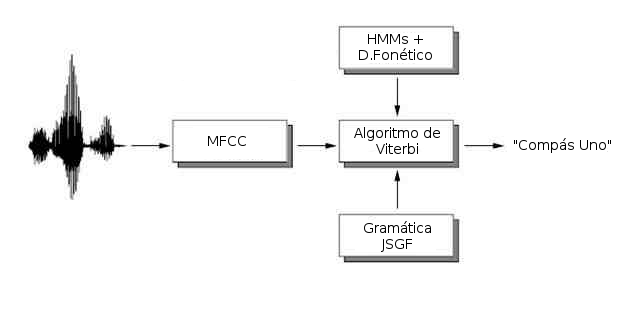
\includegraphics[width=0.7\textwidth]{./graphics/pocketsphinx.png}
\caption{Reconocimiento del habla mediante PocketSphinx. Basado en \cite{VerenichASR}.}
\label{figure:hmm}
\end{figure}
\end{frame}

\begin{frame}{Soluci\'on Propuesta (4)}
\framesubtitle{Voxforge}
\foreign{Voxforge}\cite{Voxforge} es un proyecto que busca recopilar grabaciones de voz de modo a crear 
y ofrecer varios corpus de habla bajo una licencia que permita su libre utilizaci\'on. 

El modelo ac\'ustico utilizado tiene como base las grabaciones de \foreign{Voxforge} en idioma espa\~nol,
y se encuentra disponible entre los recursos del proyecto \foreign{Pocketsphinx} para su utilizaci\'on
con el motor de reconocimiento del habla.
\end{frame}

\begin{frame}{Soluci\'on Propuesta (5)}
\framesubtitle{TamTam Listens}
\emph{TamTam Listens}, la interfaz mediante voz implementada, permite al usuario componer una 
pieza musical mediante la utilizaci\'on de tres tipos de comandos de voz:

\begin{itemize}
    \item Comandos Generales (G)
    \item Comandos de Pista (P)
    \item Comandos de Comp\'as (C)
\end{itemize}
 

\end{frame}

\begin{frame}{Soluci\'on Propuesta (6)}
\framesubtitle{TamTam Listens. Arquitectura}

\begin{figure}[H] 
\centering

\includegraphics[width=0.7\textwidth]{./graphics/tamtam-listens-arq.png}
\caption{Arquitectura b\'asica de \emph{TamTam Listens}}
\label{figure:tamtam-listens-arq}
\end{figure}

Como sugiere la figura~\ref{figure:tamtam-listens-arq}, \emph{TamTam Listens} a\~nade soporte de 
reconocimiento del habla a \emph{TamTam Edit} utilizando la librer\'ia \emph{PocketSphinx}. 
Los resultados del reconocimiento de comandos de voz son expuestos como 
un  servicio de \emph{D-Bus}\cite{Dbus2013}
La arquitectura propuesta, implementada como parte de \emph{TamTam Listens}, favorece la modularidad
y la reutilizaci\'on de la soluci\'on para otros proyectos de caracter{\'\i}sticas similares.
\end{frame}

\begin{frame}[fragile]{Soluci\'on Propuesta (7)}
\framesubtitle{TamTam Listens. Gram\'atica}
Los comandos soportados por la aplicación se definieron mediante el modelo de lenguaje, basado
en una gram\'atica en formato JSGF \cite{JSGF2000}. 

\begin{figure}[H]
\begin{lstlisting}[frame=single]
#JSGF V1.0;
grammar tamtam;

public <tamtam-listens> =  <comando>    |
    <pagina> | <pista-a> | <pista-b>    | 
    <seleccionar-compas> | <crear-nota> |
    <seleccionar-nota>   | <volumen>    |
    <duplicar-nota>      | <tempo>      | 
    <configurar-nota>    |<borrar-nota> |
    <loop>;

<comando>     = REPRODUCIR MUSICA       |
    PAUSAR MUSICA   | PARAR MUSICA      | 
    GENERAR MUSICA  | CREAR NUEVA MUSICA| 
    EXPORTAR MUSICA | SALIR DE TAMTAM;

<loop>   = (COMODIN)+;
\end{lstlisting}
\caption{Fragmento de la gram\'atica utilizada en \emph{Tamtam Listens}.}
\label{figure:fragmento-gram}
\end{figure}
\end{frame}

\begin{frame}[fragile]{Soluci\'on Propuesta (8)}
\framesubtitle{TamTam Listens. Diccionario}
Para poder mapear los fonemas reconocidos por el modelo ac\'ustico a palabras v\'alidas del dominio de la 
aplicaci\'on, \emph{PocketSphinx} utiliza un diccionario que define la secuencia de fonemas de 
cada palabra del lenguaje.

\begin{figure}[H]
\begin{lstlisting}[frame=single]
REPRODUCIR RR E P R O D U S I R
PAUSAR P A U S A R
PARAR  P A R A R
PARTITURA P A R T I T U R A
SIGUIENTE S I G I E N T E
ANTERIOR A N T E R I O R
COMODIN   A
COMODIN(2)  B
COMODIN(3)  C
COMODIN(4)  CH
\end{lstlisting}
\caption{Fragmento del diccionario fon\'etico utilizado en \emph{Tamtam Listens}.}
\label{figure:fragmento-dic}
\end{figure}
\end{frame}
